% -*- coding: utf-8 -*-
\documentclass[compress,usepdftitle=false,xcolor=pdftex,dvipsnames,table,aspectratio=169]{beamer}
\usepackage{appendixnumberbeamer}% End page count before \appendix
\usepackage{etex}
\usepackage[utf8]{inputenc} % The encoding
%\usepackage[11pt]{moresize}% More font sizes
\usepackage{eulervm}% Euler VM as math serif font

\usepackage{etoolbox}% Needed for toggles

%%%%%%%%%%%%%%%%%%%%%%%%%%%%%%%%%%%%%%%%%%%%%%%%%%%%%%%%%%%%%%%%%%%%%%%%%%%%%%%
%% Setup
%%% The bibliography
% \usepackage[style=authoryear]{biblatex}
% \bibliography{scalas-rebac-ref-rev}

\usepackage{amsmath}
%\usepackage{mathabx} % Beware: may cause compilation problems
\def\rightSquigarrow{\mathrel{\mathlarger{\mathlarger{\rightsquigarrow}}}}
\usepackage{stmaryrd}
%\usepackage{cmll} % \bigwith
% \usepackage{figlatex} % Adds .fig support for \includegraphics

%\usepackage{multirow}
\usepackage{nicefrac}               % Nice fractions
%\usepackage{colonequals} % More symbols (colon equalities)
\usepackage{multirow}% Multirows in tables

\usepackage{relsize} % Relative scaling of text/math

%\usepackage{fixltx2e} % Text mode subscript and superscript
\usepackage{xspace} % Smart spaces after commands
\usepackage{xifthen} % Extended conditional commands

%\usepackage{MnSymbol}% \llangle, \rrangle and other parentheses & symbols
\usepackage{pifont}% Fancy dingbats

\usepackage{tikz}                   % For comic-like balloons
\usetikzlibrary{matrix, positioning, shapes, arrows,
  decorations.markings, automata}
% \usetikzlibrary{calc,shapes.callouts,shapes.arrows}

\usepackage[absolute,overlay]{textpos} % Absolute placement of blocks

%\usepackage[inference]{semantic}    % Helper package for semantics
\usepackage{proof}                  % Logic proofs

\usepackage{ulem} % For strikeout effect
%\usepackage{listings}

\usepackage{transparent} % Transparent text (e.g. in Inkscape-generated images)

% \usepackage{verbatim}

% \usepackage{wasysym} % for smileys

\usepackage{pdfpages}% To include pages from an external PDF file

\usepackage{mathtools} % \xRightArrow and stuff - load late to avoid conflicts

% % Comic-like balloons, arrows etc.
% \newcommand{\arrowthis}[2]{
%         \tikz[remember picture,baseline]{\node[anchor=base,inner sep=0,outer sep=0]%
%         (#1) {{#1}};
%         \node[overlay,single arrow,draw=none,fill=red!50,anchor=tip,rotate=60] 
%         at (#1.south) {#2};}%
%     }%
% \newcommand{\bubblethis}[2]{
%         \tikz[remember picture,baseline]{\node[anchor=base,inner sep=0,outer sep=0]%
%         (#1) {{#1}};\node[overlay,cloud callout,callout relative pointer={(0.2cm,-0.7cm)},%
%         aspect=2.5,fill=yellow!90] at ($(#1.north)+(-0.5cm,1.6cm)$) {#2};}%
%     }%
% \newcommand{\speechthis}[2]{
%         \tikz[remember picture,baseline]{\node[anchor=base,inner sep=0,outer sep=0]%
%         (#1) {{#1}};\node[overlay,ellipse callout,fill=blue!50] 
%         at ($(#1.north)+(-.5cm,0.8cm)$) {#2};}%
%     }%
% \newcommand{\pointthis}[2]{
%         \tikz[remember picture,baseline]{\node[anchor=base,inner sep=0,outer sep=0]%
%         (#1) {{#1}};\node[overlay,rectangle callout,%
%         callout relative pointer={(0.2cm,0.7cm)},fill=green!50] at ($(#1.north)+(-.5cm,-1.4cm)$) {#2};}%
%         }%

%%%%%%%%%%%%%%%%%%%%%%%%%%%%%%%%%%%%%%%%%%%%%%%%%%%%%%%%%%%%%%%%%%%%%%%%%%%%%%%
% Workaround to make \pause behave correctly inside alignments
%
% See:
%
% http://tex.stackexchange.com/questions/6348/problem-with-beamers-pause-in-alignments
%%%%%%%%%%%%%%%%%%%%%%%%%%%%%%%%%%%%%%%%%%%%%%%%%%%%%%%%%%%%%%%%%%%%%%%%%%%%%%
\makeatletter
\def\beamerorig@set@color{%
  \pdfliteral{\current@color}%
  \aftergroup\reset@color
}
\def\beamerorig@reset@color{\pdfliteral{\current@color}}
\makeatother
%%%%%%%%%%%%%%%%%%%%%%%%%%%%%%%%%%%%%%%%%%%%%%%%%%%%%%%%%%%%%%%%%%%%%%%%%%%%%%%

% Highlighting
\newcommand{\HLight}[1]{{\setlength{\fboxsep}{0pt}\colorbox{yellow}{#1}}}
\newcommand{\HLightB}[1]{{\setlength{\fboxsep}{0pt}\colorbox{Lavender!50}{#1}}}
% \newcommand{\OKLight}[1]{{\setlength{\fboxsep}{0pt}\colorbox{green}{#1}}}
% \newcommand{\KOLight}[1]{{\setlength{\fboxsep}{0pt}\colorbox{gray}{#1}}}
\newcommand{\OKmark}{\ensuremath{{\huge{\color{Green}\text{\ding{51}}}}}}%
\newcommand{\KOmark}{\ensuremath{{\huge{\color{Red}\text{\ding{55}}}}}}%
\newcommand{\smallOKmark}{\ensuremath{{\Large{\color{Green}\text{\ding{51}}}}}}%

\definecolor{hlight}{rgb}{0.99, 0.95, 0.80}
\setbeamercolor{hlightBox}{bg=hlight}
\setbeamercolor{yellowBox}{bg=yellow}

\newcommand{\bluebf}[1]{{\textbf{\color{blue}#1}}}%
\newcommand{\redbf}[1]{{\textbf{\color{red}#1}}}%
\newcommand{\greenbf}[1]{{\textbf{\color{OliveGreen}#1}}}%
\newcommand{\brownbf}[1]{{\textbf{\color{Brown}#1}}}%

% Horizontal separator
\newcommand{\myRule}{%
  \vspace{-0.3cm}
  {\color{Gray}\rule{\textwidth}{1pt}}
  \vspace{-0.2cm}
}%

% Strikeout
\newcommand\redout{%
  \bgroup\markoverwith{\textcolor{Red}{\rule[0.4ex]{10pt}{4pt}}}\ULon%
}

%\usetheme[subsection=false]{Dresden}
\useoutertheme[subsection=false]{miniframes}
\usefonttheme{professionalfonts}
\setbeamercolor{section in head/foot}{fg=white, bg=black}
% \setbeamercolor{mini frame}{fg=white, bg=black}
\usefonttheme[onlylarge]{structurebold}
%\setbeamerfont*{frametitle}{size=\normalsize,series=\bfseries}
\setbeamertemplate{navigation symbols}{}
%\setbeamertemplate{headline}[miniframes theme]{}
%\setbeamertemplate{footline}[default]
\setbeamertemplate{footline}[frame number]

%%\usecolortheme{whale}

%\setbeamercovered{transparent=20}

\normalem % Don't mess with \em and \emph!

%% Squeeze bibliography style
\setbeamertemplate{bibliography entry title}{}
\setbeamertemplate{bibliography entry location}{}
\setbeamertemplate{bibliography entry note}{}

%\usepackage{fancyvrb}% Required by pygments.tex below
%\input{pygments.tex}% Autogenerated by Makefile

%% Macro definitions
\input{macros.tex}
%x\newcommand{\putat}[3]{\begin{picture}(0,0)(0,0)\put(#1,#2){#3}\end{picture}}

%%%%%%%%%%%%%%%%%%%%%%%%%%%%%%%%%%%%%%%%%%%%%%%%%%%%%%%%%%%%%%%%%%%%%%%%%%%%%%%
%% Title
\def\myTitlePlain{Distributed clouds --- $\mu$ clouds}%
\def\myTitle{Distributed clouds --- $\mu$ clouds}

\hypersetup{
  pdfauthor={Milo\v s Simi\' c},
  pdftitle={\myTitlePlain},
  pdfkeywords= {cloud computing} {distributed systems} {micro clouds} {distributed clouds},
}

\title{%
  \\[8mm]%
  \huge%
  \myTitle%
}%

\institute[University of Novi Sad, Serbia]{}

\author{%
  \vspace{-1mm}%
  \centering%
  {{\underline{\bluebf{Short introdiction, and other interesting bits and pieces}}}}%
  \quad
  \\[7mm]%
  \scalebox{0.8}{%
  \begin{minipage}{1.2\linewidth}
  \centering%
  %\raisebox{-6mm}{%
    \includegraphics[height=12mm]{images/novi-sad.pdf}%
    \raisebox{2mm}{
      \begin{minipage}[b]{0.30\linewidth}
        \bf%
        University of Novi Sad\\
        Faculty of Technical Sciences
      \end{minipage}
    }% end \raisebox
  \end{minipage}
  }% end \scalebox
  \vspace{-0mm}%
}% end \author

\date{%
}% end \date

\newcommand{\quickCite}[1]{{\scriptsize\color{gray}(#1)}}

%%%%%%%%%%%%%%%%%%%%%%%%%%%%%%%%%%%%%%%%%%%%%%%%%%%%%%%%%%%%%%%%%%%%%%%%%%%%%%%

 

\begin{document}

\frame[plain]{%
  \titlepage%
}

\setcounter{framenumber}{0}%

\section{Intro}%
\subsection{Intro}%

\begin{frame}
	\frametitle{Table of concent}
	
	\begin{itemize}
		
		\item Enormously striped down intro to distributed systems --- to follow rest of the talk
		\item Short explanation of cloud infrastructure and its problems --- more basics
		\item Distributed clouds and micro cloud model --- overall idea
		\item Current work and possibilities for you
		\item Conclusion
		\item Questions and Discussions
		
	\end{itemize}
	
\end{frame}

\begin{frame}
	\frametitle{Who am I, and why am I here}
	
	\begin{columns}
		\begin{column}{0.5\linewidth}
			\begin{itemize}
				\item PhD to be, 18 published papers (3 in SCI journals --- 2/3 M21)
				\item Best paper award, 2013, (academia)
				\item ThinkX in the category Community and Social Impact, 2018, (industry)
				\item Invited lecture, Imperial College London, 2021, (academia)
				\item Fields of interest: distributed systems, (multi) cloud computing, big data, microservices, NoSQL engines, probabilistic data structures
				\item Misinformation: doing something in IoT area
			\end{itemize}
		\end{column}
		\begin{column}{0.5\linewidth}
			\includegraphics[width=1\linewidth,angle=270,origin=c]{images/me}
		\end{column}
	\end{columns}
	
\end{frame}

\section{Distributed systems}%
\subsection{Distributed systems}%

\begin{frame}
	\frametitle{Distributed systems}
	
	\begin{itemize}
		\item There are various definitions of distributed systems
		\item We can think of distributed system as a system where multiple entities can communicate to one another in some way, but at the same time, they can perform some operations
		\item Andrew Tanenbaum gives two interesting assumptions:~\quickCite{Distributed systems - principles and paradigms, 2nd Edition}:
		\begin{enumerate}
			\item  \emph{A computing element, which we will generally refer to as a node, can be either a hardware device or a software process};
			\item \emph{A second element is that users (be they people or applications) believe they are dealing with a single system --- this means that one way or another the autonomous nodes need to collaborate}.
		\end{enumerate}
	\end{itemize}
	
\end{frame}

\begin{frame}
	
	\begin{itemize}
		\item Three significant characteristics of distributed systems are:~\quickCite{Distributed systems - principles and paradigms, 2nd Edition}:
		\begin{enumerate}
			\item \textbf{Concurrency of components}, refers to the ability of the distributed system that multiple activities are executed at the same time. These activities take place on multiple nodes that are part of a distributed system;
			\item \textbf{Independent failure of components}, this property refers to a nasty feature of distributed system that nodes fail independently. They can fail at the same time as well, but they usually fail independently for numerous reasons;
			\item \textbf{Lack of a global clock}, this is a consequence of dealing with independent nodes --- each node has its notion of time, and as such we cannot assume that there is something like a global clock.
		\end{enumerate}
	\end{itemize}
	
\end{frame}

\begin{frame}
	
	\begin{itemize}
		\item Distributed systems existed before computers started to enrich/complicate almost every aspect of human life
		\item Distributed systems have been used in various different domains such as: \textbf{telecommunication networks}, \textbf{aircraft control systems}, \textbf{industrial control systems}, etc.
		\item Distributed systems are used anywhere where the number of users is growing rapidly so that a single entity cannot respond to the demands in (near) real-time
		\item Distributed systems (in computer science) consist of various algorithms, techniques, and trade-offs to create an \textbf{illusion} that a set of nodes act as one
		\item Algorithms and techniques used in the distributed systems may include the following: \textbf{(1)} replication, \textbf{(2)} consensus, \textbf{(3)} communication, \textbf{(4)} storage,\textbf{(5)} processing, \textbf{(6)} \textbf{membership}, \textbf{(7)} scheduling etc.
	\end{itemize}
	
\end{frame}

\begin{frame}
	\frametitle{Scalability}
	
	\begin{itemize}
		\item Scalability is the property of a system to handle a growing amount of work by adding resources to the system~\quickCite{Characteristics of scalability and their impact on performance}
		\item When talking about computer systems, scalability can be represented in two ways:
		\begin{enumerate}
			\item \textbf{Scaling vertically} means upgrading the hardware that computer systems are running on (bounded by Moore's law) --- usually high end hardware
			\item \textbf{Scaling horizontally} means that we scale our system by adding more and more computers (almost limitless on how much we can scale) --- commodity hardware
		\end{enumerate}
		\item Scaling horizontally is a preferable way for scaling distributed systems, it is significantly cheaper allowing fault tolerance and low latency, \textbf{but} it requers specific programming mindset --- \textbf{accepts the failure, and deal with it!}
	\end{itemize}
	
\end{frame}

\begin{frame}
	\frametitle{Clusters}
	
	\begin{itemize}
		\item Nodes are usually organized into groups of machines working together and/or on the same goal --- \textbf{clusters}
		\item Spreading workload and/or applications on them
		\item Cluster can be described as a processing system, which consists of a collection of interconnected stand-alone computers cooperatively working together as a single, integrated computing resource~\quickCite{Distributed data stream processing and edge computing: A survey on resource elasticity and future directions}
		\item Spreading storage on multiple nodes leads to \textbf{C}onsistency, \textbf{A}vailability, \textbf{P}artitioning (CAP) theorem ---  it is impossible for a distributed store to simultaneously provide more than two out of three guarantees (and in distributed setup P we cannot eliminate)~\quickCite{Towards Robust Distributed Systems, Brewer's conjecture and the feasibility of consistent, available, partition-tolerant web services}
		\item CRDTs tackle this, but more about it some other time~\quickCite{Conflict-free Replicated Data Types (CRDTs)}
	\end{itemize}
	
\end{frame}

\section{Cloud computing}%
\subsection{Cloud computing}%

\begin{frame}
	\frametitle{Cloud computing}
	
	Cloud is usually depicted as a pyramid of offered services something like:
	\begin{columns}
		\begin{column}{0.5\linewidth}
			\begin{itemize}
				\item Nice for marketing, and marketing only
				\item Hides the complexity, but good for presentations
				\item From the engineering perspective, we still have no idea how this thing works, and what we can expect!
				\item Usually leads to writing hateful comments on twitter :)
				\item * as a service (nonsense)
			\end{itemize}
		\end{column}
		\begin{column}{0.5\linewidth}
			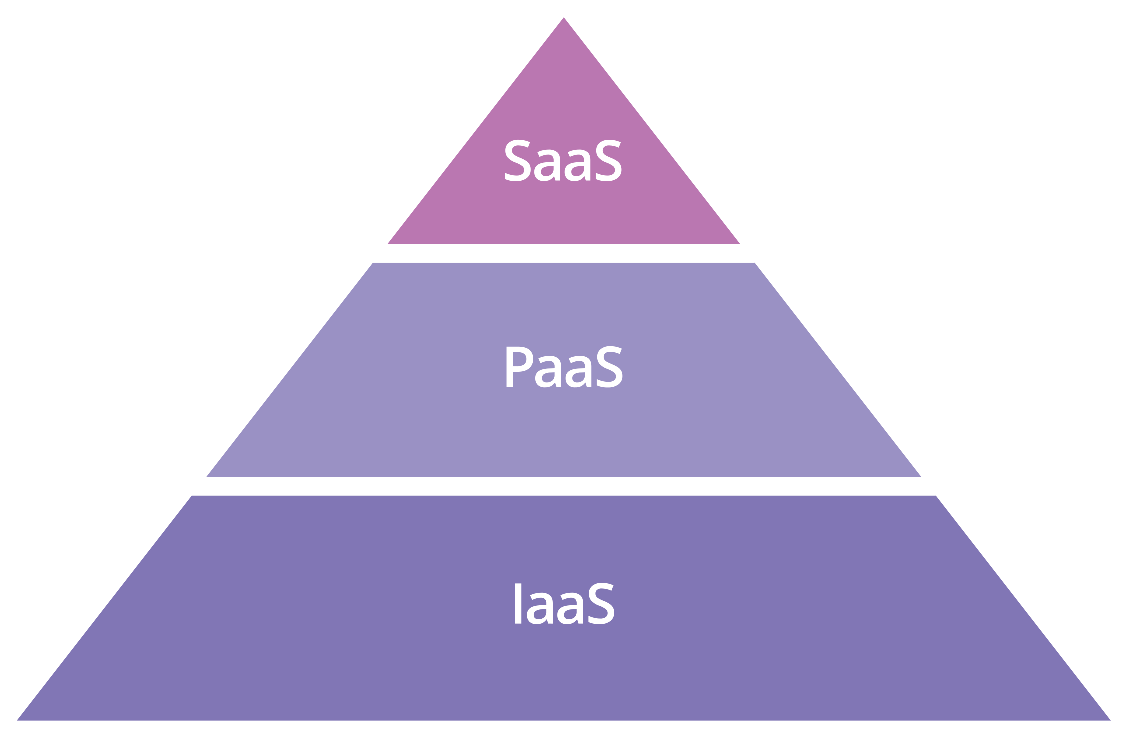
\includegraphics[width=1\linewidth]{images/pyramid}
		\end{column}
	\end{columns}
	
\end{frame}

\begin{frame}
	\frametitle{Cloud computing --- take 2}
	
	If we are favoring one provider over the other we might end up here:
	\begin{columns}
		\begin{column}{0.5\linewidth}
			\begin{itemize}
				\item Nice for fans, and fans only
				\item From the engineering perspective, we still have no idea how this thing works, and what we can expect!
				\item Usually leads to writing even more hateful comments on twitter :)
				\item People expect that cloud provider will solve all their problems
				\item A dream: \emph{framework will solve all our problems} --- short answert \textbf{it will not!}
			\end{itemize}
		\end{column}
		\begin{column}{0.5\linewidth}
			\includegraphics[width=0.9\linewidth]{images/aws}
		\end{column}
	\end{columns}
	
\end{frame}

\begin{frame}
	\frametitle{Third time’s a Charm --- an engineering point of view}
	
	\emph{There is no cloud just someone else's computer}
	
	\begin{columns}
		\begin{column}{0.5\linewidth}
			\includegraphics[width=1\linewidth]{images/building}
		\end{column}
		\begin{column}{0.5\linewidth}
			\includegraphics[width=1\linewidth]{images/clusters}
		\end{column}
	\end{columns}
	
	And we need to have the way to program these clusters of machines
	
\end{frame}

\begin{frame}
	\frametitle{Cloud architecture}
	
	\begin{itemize}
		\item The first building block of cloud architecture is a \textbf{cluster} --- a set of nodes or servers (resources) that operate as a single unit to achieve some goal
		\item The next building block that consists of multiple clusters is called a \textbf{regions (or data centers)} --- isolated and independent from each other, containing resources in form of clusters
		\item Regions are usually composed of a few \textbf{availability zones}~\quickCite{QVIA-SDN: Towards QoS-Aware Virtual Infrastructure Allocation on SDN-based Clouds} --- defense against the fail
		\item If for whatever reason, one zone fails or goes offline, there are still more of them to serve user requests --- better availability, scalability, and resilience
	\end{itemize}
	
\end{frame}

\begin{frame}
	\frametitle{Membership protocol}
	
	\begin{itemize}
		\item The most basic task is that all nodes need to answer --- which group they belong to, and who are their peers in the group they will collaborate with
		\item In the setup where nodes are connected over the local network or internet, and they need to communicate, things \textbf{will} go wrong for various reasons
		\item \emph{Bad things happen to good nodes. A tale of distributed systems}
		\item To resolve the problem who their group peers are, a \textbf{membership protocol} comes to help
		\item Processes in the group of nodes will ping each other in different ways, using different strategies to figure out which nodes are \textbf{dead} and which are \textbf{alive}
		\item This give us two interesting features: \textbf{Failure detection}, and \textbf{Information dissemination}
	\end{itemize}
	
\end{frame}

\begin{frame}
	\frametitle{SWIM}
	
	\begin{center}
		\includegraphics[width=0.7\linewidth]{images/Figure15}\\
	\end{center}
	Try direct ping, if you do now get ACK; ask someone else to probe it for you; if still no ACK, suspect dead; eventually, declare dead~\quickCite{SWIM: Scalable Weakly-consistent Infection-style Process Group Membership Protocol}
\end{frame}

\begin{frame}
	\frametitle{What is the cloud then?}
	
	\begin{itemize}
		\item Vogels et al. describe cloud computing as an \textbf{aggregation of computing resources as a utility, and software as a service}~\quickCite{A head in the clouds the power of infrastructure as a service}
		\item Big data centers provide hardware and software services for their users over the internet~\quickCite{Above the Clouds: A Berkeley View of Cloud Computing}
		\item Cloud providers offer various resources like CPU, GPU, storage, and network as utilities that can be used and released on-demand~\quickCite{Cloud computing: state-of-the-art and research challenges}
		\item Cloud computing relies on \textbf{centralization of resources} --- offering them to users elastically
	\end{itemize}
	
\end{frame}

\begin{frame}
	\frametitle{Cloud infrastructure costs}
	
	\begin{columns}
		\begin{column}{0.5\linewidth}
			\begin{itemize}
				\item Centralization relies on the \textbf{economy of scale} --- lower the administration costs
				\item Organizations using cloud services avoid huge investments --- creating and maintaining their own data centers
				\item They consume cloud resources and pay for usage time --- \emph{pay as you go model}~\quickCite{The Emergence of Edge Computing}
				\item Data \textbf{must} to be moved to the cloud --- introduces high latency~\quickCite{Edge computing framework for enabling situation awareness in IoT based smart city} 
			\end{itemize}
		\end{column}
		\begin{column}{0.5\linewidth}
			\begin{center}
				\includegraphics[width=1\linewidth]{images/costs}\\
				\quickCite{https://perspectives.mvdirona.com/2008/11/cost-of-power-in-large-scale-data-centers/}
			\end{center}
		\end{column}
	\end{columns}
	
\end{frame}

\begin{frame}
	\frametitle{Services}
	
	\begin{itemize}
		\item Services are built in such a way to (fully) utilize this infrastructure
		\item Cloud-native (containers, scheduled, traceing, rpcs, events, ....)
		\item Service oriented applications (microservices is a buzz $\neq$ distributed system --- it is an application model)
		\item (hmmm) Easy to scale, operate in multiple places
		\item All should be automated!!!!!
		\item Usually use some storage system, which is able to scale well on a lot of nodes
		\item On top of this, the users run their own applications with (almost) similar capabilities --- learn from the best
	\end{itemize}
	
\end{frame}

\begin{frame}
	\frametitle{Cloud computing problems}
	
	\begin{itemize}
		\item Centralization, and demand to move all data to cloud is one big issue
		\begin{itemize}
			\item Boeing 787s per single flight generates \textbf{half a terabyte of data}~\quickCite{Edge Computing: A Primer}
			\item A self-driving car generates \textbf{two petabytes of data per single drive}~\quickCite{Edge Computing: A Primer}
		\end{itemize}
		\item On the other hand, bandwidth is not large enough to support such requirements~\quickCite{Edge Computing: A Primer}
		\item Some applications require real-time processing for proper decision-making, e.g. self-driving cars, delivery drones, power balancing in electric grids, patient health monitoring, etc.
		\item Such applications might face \textbf{serious issues} if a cloud service becomes unavailable due to whatever reason~\quickCite{Why Does the Cloud Stop Computing? Lessons from Hundreds of Service Outages}.
	\end{itemize}
	
\end{frame}

\section{Distributed clouds}%
\subsection{Distributed clouds}%

\begin{frame}
	\frametitle{Distributed clouds}
	
	\begin{itemize}
		\item The cloud is usually far away from end devices because data centers are built on specific locations in the world to target as many users nearby as possible
		\item This sparse deployment will most likely lead to high latency, and bad quality of experience (QoE)~\quickCite{Computation Offloading Toward Edge Computing} for most users
		\item Latency-sensitive applications \textbf{especially} will have a hard time
		\item Relax the cloud a little bit, and move some tasks from the cloud, opening the door for next gen models
		\item Fog computing, edge computing, osmotic computing, cloudlets, ....
		\item Models where computing and storage resources are in \textbf{proximity to data sources}~\quickCite{The Emergence of Edge Computing}
	\end{itemize}
	
\end{frame}

\begin{frame}
	\frametitle{Next gen}
	
	\begin{center}
		\includegraphics[width=0.6\linewidth]{images/matrix}\\
		\quickCite{Cloud Native Maturity Matrix}
	\end{center}
	
\end{frame}

\begin{frame}
	\frametitle{Edge computing}
	
	\begin{itemize}
		\item Edge computing introduced \textbf{small-scale servers} that operate \textbf{between data sources and the cloud}
		\item These small-scale servers have much fewer capabilities compared to the cloud servers~\quickCite{On the computation offloading at ad hoc cloudlet: architecture and service modes}
		\item To avoid latency and huge bandwidth, edge computing nodes can be dispersed in various locations, for example, base stations~\quickCite{A heterogeneous mobile cloud computing model for hybrid clouds, A Survey on Mobile Edge Networks: Convergence of Computing, Caching and Communications}, restaurants, or over arbitrary geographic regions.
		\item Nearby nodes could be \textbf{organized locally}, making the whole system more available and reliable --- extending resources beyond the single node or group of nodes, maintaining good performance to build servers and clusters~\quickCite{Towards green data centers: {A} comparison of x86 and {ARM} architectures
			power efficiency}.
	\end{itemize}
	
\end{frame}

\begin{frame}
	\frametitle{Clusters}
	
	\begin{columns}
		\begin{column}{0.5\linewidth}
			\includegraphics[width=0.8\linewidth]{images/arm}
		\end{column}
		\begin{column}{0.5\linewidth}
			\includegraphics[width=1\linewidth]{images/clusters}
		\end{column}
	\end{columns}

\begin{center}
	Clusters of commodity hardware, arm k8s clusters are real --- \HLightB{when there's a cluster there's a way}
\end{center}

\end{frame}

\begin{frame}
	\frametitle{Related work}
	
	\begin{itemize}
		\item Platform models:
		\begin{itemize}
			\item Kubernetes --- an (updated) open-source variant of Google orchestrator Borg
			\item Nebula
			\item OpenStack
		\end{itemize}
	\item Nodes organization:
	\begin{itemize}
		\item Zone-based organization~\quickCite{A zone-based content pre-caching strategy in vehicular edge networks}
		\item Micro data centers --- serve nearby population (theory)
		\item Nano data centers --- serve single household (using SDN)
		\item Drop computing --- ad hoc formation~\quickCite{Drop computing: Ad-hoc dynamic collaborative computing}
	\end{itemize}
	\item Processing:
	\begin{itemize}
		\item \textbf{data locality} --- moving computation to the data, minimizing network congestion~\quickCite{Investigation of Data Locality in MapReduce}
		\item Lambda architectures~\quickCite{Lambda architecture for cost-effective batch and speed big data processing}
	\end{itemize}
	\end{itemize}

\end{frame}

\begin{frame}
	\frametitle{Small data centers}
	
	\begin{itemize}
		\item Greenberg et al. introduce the idea of micro data centers as data centers that operate in proximity~\quickCite{The cost of a cloud: research problems in data center networks} 
		\item Their minimum size is defined by the needs of the local population, as such, they are reducing traditional data centers fixed costs~\quickCite{The cost of a cloud: research problems in data center networks, Mobile Edge Computing: A Survey}
		\item The main feature micro data centers are relying on is agility --- ability to dynamically grow and shrink resources to satisfy the resource demands from the most optimal location~\quickCite{The cost of a cloud: research problems in data center networks}
		\item We can go even smaller using a network of gateways equipped with some storage, for internet services at home forming even smaller  data centers -- nano data centers~\quickCite{Cost-Effective Content Delivery Networks Using Clouds and Nano Data Centers}
		\item There are possible usage for these data centers in some large scale applications with much less energy consumption than traditional data centers
	\end{itemize}
	
\end{frame}

\begin{frame}
	\frametitle{Connecting the dots}
	
	\begin{itemize}
		\item On the high level, the cloud architecture is separated into few building blocks that make the whole system lot easier to understand, maintain and operate --- clusters, regions, availability zones
		\item We can observe \textbf{micro clouds} as \emph{geo-distributed systems with dispersed users}~\quickCite{Beyond The Clouds, How Should Next Generation Utility Computing Infrastructures Be Designed?}, we can use a similar model with some adaptations
		\item Geo-distribution means in proximity to some large populations, where micro clouds serve user requests locally first
		\item Rely on a similar proven strategy, do not build the entire new model, but adapt the existing one for the different use-cases
		\item Forming micro data centers or nano data centers (pools of resources) depends on usage and local population size
	\end{itemize}
	
\end{frame}

\begin{frame}
	\frametitle{Organization of the nodes}
	
	\begin{itemize}
		\item Group of nodes virtually and/or geographically separated, that works together to provide the same service to clients, form a \textbf{cluster}
		\item A concept used to describe a set of clusters (that could be) scattered over an arbitrary geographic region, forms a \textbf{region}
		\item Highest logical concept that is composed of a minimum of one region and could span over multiple regions is \textbf{topology}
		\item \textbf{To lower the latency, the vast distances between clusters should be strongly avoided in normal circumstances!}
	\end{itemize}
	
	\bigskip
	
	\begin{table}[h!]
		\begin{center}
			\begin{tabular}{l|l}
				\textbf{Edge centric computing} & \textbf{Cloud computing}\\
				\hline
				Topology (logical) & Cloud provider (logical)\\
				Region (logical) & Region (physical)\\
				Cluster (physical) & Zone (physical)\\
			\end{tabular}
		\end{center}
		\caption{Similar concepts between cloud and edge-centric computing}
		\label{tab:table1}
	\end{table}
	
\end{frame}

\begin{frame}
	\frametitle{Edge-centric computing as a service architecture with separation of concerns}
	
	\begin{figure}[H]
		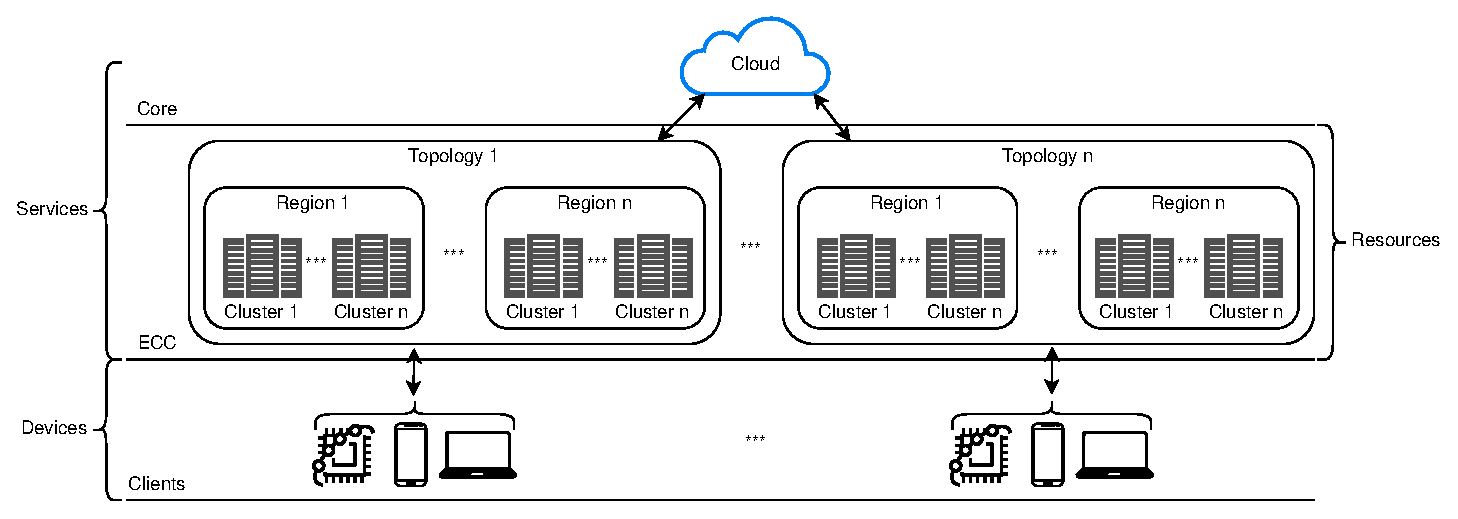
\includegraphics[width=\linewidth]{images/FIG1}
	\end{figure}
\end{frame}

\begin{frame}
	\frametitle{Micro clouds}
	
	\begin{columns}
		\begin{column}{0.5\linewidth}
			\begin{itemize}
				\item Ephemeral cloud-like structures serving local requests first, before reaching to the traditional cloud 
				\item Their size and existence are defined by the local population using them
				\item Clients have illusion that communicate with the traditional clouds
				\item Designed for failure using automated tools where no micro cloud is irreplaceable
				\item Colaboration between cloud computing and edge computing
			\end{itemize}
		\end{column}
		\begin{column}{0.5\linewidth}
			\includegraphics[scale=0.7]{images/Figure9}
		\end{column}
	\end{columns}

\end{frame}

\begin{frame}
	\frametitle{Physical capabilities}
	\begin{itemize}
		\item Capabilities of ARM-based devices have a good performance for building servers and clusters, considering their performance per Watt relation \quickCite{Aroca \emph{et al.}, J. Parallel Distributed Comput., 2012}
		\item These servers can be spread in base stations, coffee shops, or over geographic regions to avoid latency, and huge bandwidth \quickCite{Wang \emph{et al.}, IEEE Access, 2017, Monsalve \emph{et al.}, Future Gener. Comput. Syst., 2018}
		\item They can serve as firewalls and pre-processing tier for the cloud \quickCite{Satyanarayanan\emph{et al.}, EDGE 2019}
		\item Users get a unique ability to dynamically and selectively control the information sent to the cloud \quickCite{Satyanarayanan\emph{et al.}, EDGE 2019}
	\end{itemize}
\end{frame}

\begin{frame}
	\frametitle{So what's new?}
	
	\begin{itemize}
		\item The existing orchestrator engines (e.g., Kubernetes, Apache Mesos, Docker Swarm, etc.) operate one cluster level~\quickCite{Borg, Omega, and Kubernetes, Running in multiple zones}, and cluster could span over multiple availability zones
		\item Kubernetes allow multi-cluster deployments~\quickCite{Running in multiple zones}, handling these clusters as disposable --- "treating \textbf{clusters} as cattle, not pets" (i.e., numerous servers/clusters built using automated tools designed for failure, where no servers/clusters are irreplaceable~\quickCite{Review of CERN Data Centre Infrastructure}).
		\item The model we proposed goes one step further, allowing the creation of numerous micro clouds designed for failure using automated tools where no micro clouds is irreplaceable --- "treating \textbf{micro couds} as cattle, not pets."
		\item Such an extension allows infrastructure optimization in more dimensions~\quickCite{Hierarchical Approach for Green Workload Management in Distributed
			Data Centers}
	\end{itemize}
	
\end{frame}

\begin{frame}
	\begin{itemize}
		\item Specialized models are developed and optimized for a specific use case to take the maximum out of hardware and software
		\item They might outperform the proposed model in terms of speed
		\item The proposed model allows organization and reorganization of resources in a similar way the cloud does, allowing users to develop applications without some specialized infrastructure for different applications --- more development freedom
		\item Users will be able to create new interesting human-centered applications in the future, utilizing both cloud and edge
		\item The proposed model is more oriented towards developing a broader specter of applications without the need for a specialized hardware or software
	\end{itemize}
\end{frame}

\begin{frame}
	\frametitle{Who can join the system}
	
	To be part of the system a node must satisfy four simple rules:
	\begin{enumerate}
		\item Run an operating system with a file system
		\item Be able to run some application isolation tool, for example, a container or unikernel engine
		\item Have available resources for utilization
		\item Have internet connection
	\end{enumerate}
	
	\bigskip
	
	\begin{itemize}
		\item These simple yet powerful rules could be helpful in certain situations --- increased demand for resources that the currently available infrastructure cannot support
		\item In such a scenario, the \textbf{inclusion of volunteer nodes} into the system can be allowed to depreciate load for an indefinite period
	\end{itemize}
	
\end{frame}

\begin{frame}
	\frametitle{Formation of micro clouds and the protocols} 
	
	\begin{itemize}
		\item Nodes are organized into micro clouds dynamically, abstracting infrastructure to the level of software --- infrastructure as software
		\item The system we propose uses remote configuration and it relies on three protocols:
		\bigskip 
		\begin{enumerate}
			\item health-check protocol informs the system about the state of every node --- background
			\item cluster formation protocol forms new clusters --- mutate operation
			\item list detail protocol shows the current state of the system to the user --- list operatio
		\end{enumerate}
	\end{itemize}

\end{frame}

\begin{frame}
	\frametitle{How to prove this?}
	
	\begin{columns}
		\begin{column}{0.5\linewidth}
			\begin{center}
				If there is a bug in a distributed algorithm, \\
				no matter how improbable it may seem, \\
				it's not a question of whether it will appear, \\
				it's a question of when it will appear.
			\end{center}
			\quickCite{Leslie Lamport, Heidelberg Laureate Forum 2021, https://www.youtube.com/watch?v=KVs3YFKqclU}
		\end{column}
		\begin{column}{0.5\linewidth}
			\begin{center}
				\includegraphics[scale=0.4]{images/leslie}\\
				\quickCite{Leslie Lamport, Turing award amongst others}
			\end{center}
		\end{column}
	\end{columns}
	
\end{frame}

\begin{frame}
	\frametitle{Formally specifying our protocols}
	
	\begin{columns}
		\begin{column}{0.5\linewidth}
				\begin{itemize}
				\item Formal analysis
				\item Multiparty asynchronous session types
				\item \HLightB{A true taste of computer science}
			\end{itemize}
			
			\bigskip
			
			We were searching for:
			\begin{itemize}
				\item a formalism that is proven correct
				\item and expressive enough
				\item but also easy to follow
			\end{itemize}
		\end{column}
		\begin{column}{0.5\linewidth}
			\includegraphics[width=\linewidth]{images/heidi}\\
			\quickCite{twitter.com/heidiann360/status/1332711011451867139}
		\end{column}
	\end{columns}

	\bigskip
	
	\begin{itemize}
		\item Joint work with Ivan Proki\'c and Jovana Dedei\'c from Chair of Matematics FTN
		\item Invited to present to eminent professors and colleagues from Imperial College London
	\end{itemize}

\end{frame}


\begin{frame}
	\frametitle{Possible real-life implementations}
	
	\begin{columns}
		\begin{column}{0.5\linewidth}
			We see two possible scenarios for implementation: 
			\begin{itemize}
				\item a stand-alone implementation
				\item integration within existing tools, as a node organizer and register
			\end{itemize}
		\end{column}
		\begin{column}{0.5\linewidth}
			Proof of concept implementation using open source tools --- constellations project (c12s)
			\begin{center}
				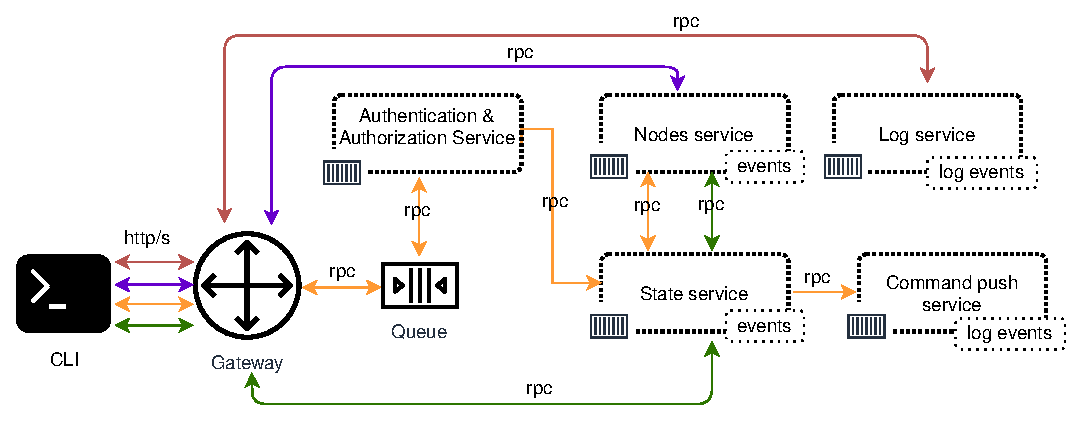
\includegraphics[width=\linewidth]{images/FIG5}
			\end{center}
		\end{column}
	\end{columns}

\bigskip
 
\quickCite{M. Simić, I. Prokić, J. Dedeić, G. Sladić and B. Milosavljević, "Towards Edge Computing as a Service: Dynamic Formation of the Micro Data-Centers," in IEEE Access, vol. 9, pp. 114468-114484, 2021, doi: 10.1109/ACCESS.2021.3104475.}

\end{frame}

\begin{frame}
	\frametitle{Remote formation is tricky}
	
	\begin{itemize}
		\item Infrastructure deployment will not happen overnight, and it might take years
		\item It might not be started at all until the whole process is trivial \quickCite{The Case for VM-Based Cloudlets in Mobile Computing}
		\item This is a complicated task~\quickCite{The future of mobile cloud computing: Integrating cloudlets and Mobile Edge Computing}
		\item Because of those properties, the key problem that needs to be resolved is how to simplify micro clouds management
		\item The naive approach would require going to every node and do it manually
		\item This process is super tedious and time-consuming, especially if we consider a geo-distributed environment
	\end{itemize}
	
\end{frame}

\begin{frame}
	\frametitle{Then how?}
	
	\begin{itemize}
		\item The infrastructure needs to be constantly deployed and maintained, so it would be beneficial to view the \textbf{infrastructure as software}~\quickCite{Infrastructure Is Software Too!}
		\item The benefit of this approach lies in the already available tools, principles, and techniques (e.g. reuse, testing, modeling, and evaluation) that can equally be used for the infrastructure definitions ~\quickCite{Software Processes Are Software Too, Revisited: An Invited Talk on the Most Influential Paper of ICSE 9, Infrastructure Is Software Too!}
		\item Presented model is moveable in between edge and cloud depending do we want our model to be more cloud-like or more edge-like
		\item To achieve such elasticity, we must abstract the infrastructure to the level of software, creating \textbf{infrastructure programming}~\quickCite{Infrastructure Is Software Too!}, allowing micro clouds infrastructure to be managed similarly as the software is
	\end{itemize}
	
\end{frame}

\begin{frame}
	
	\begin{itemize}
		\item Users specify desired state using YAML or some other format --- sorry no DSLs here
		\item Specification is done descriptively
		\item Influenced by \textbf{infrastructure as code} tools and principles like Terraform
		\item Submit \textbf{new state} to the system, and let the system deals with the rest --- \textbf{cluster formation} protocol
		\item Using \textbf{immutable infrastructure deployment} allow rolling update strategy
		\item Rolling update strategy updates large environments, a few nodes at the time
		\item Rely on containers for everything, even OS --- LinuxKit allows that Linux OS subsystems may be composed of very secure containers
		\item Unikernels (in the future maybe)
	\end{itemize}
	
\end{frame}

\begin{frame}
	\frametitle{Cluster formation protocol --- mutate operation}
	
	\begin{center}
		\includegraphics[scale=0.6]{images/FIG3}
	\end{center}
	
\end{frame}

\begin{frame}
	\frametitle{The reconciler pattern}
	
	\begin{columns}
		\begin{column}{0.5\linewidth}
			\begin{itemize}
				\item System is dealing with changes in a similar way Kubernetes does --- reconciler pattern~\quickCite{Kubernetes in Action}
				\item Tracking of resources using two simple states:
				\begin{enumerate}
					\item expected state --- desired state
					\item current state --- actual state
				\end{enumerate}
				\item The pattern runs a reconciliation loop --- ensures that the states remains the same
				\item Every node must provide his current state, simpliest way \textbf{health-check} protocol
				\item Extension is simple
			\end{itemize}
		\end{column}
		\begin{column}{0.5\linewidth}
			\begin{center}
				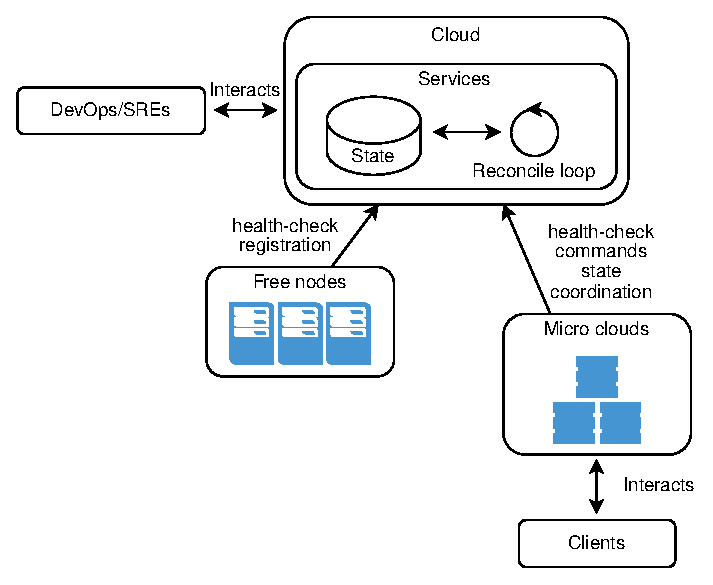
\includegraphics[scale=0.65]{images/Figure3}
			\end{center}
		\end{column}
	\end{columns}
	
\end{frame}

\begin{frame}
	\frametitle{Health-check protocol}
	
	\begin{center}
		\includegraphics[scale=0.8]{images/FIG2}
	\end{center}
	
\end{frame}

\begin{frame}
	\frametitle{Who operate micro clouds}
	
	\begin{itemize}
		\item SREs are the ones dealing with pools of resources and programmable infrastructure --- organizing and repurposing micro cloud infrastructure, as well as monitoring and managing remote configuration and uptime
		\item DevOps engineers may set up their infrastructure for continuous delivery, application metrics, etc. to deploy services and applications that users may utilize
		\item Developers develop their applications usuall way
	\end{itemize}
	
\end{frame}

\begin{frame}
	\frametitle{Applications}
	
	\begin{columns}
		\begin{column}{0.5\linewidth}
			
			\begin{itemize}
				\item All existing applications in the cloud can be upgraded to use new model
				\item Big data applications - preprocessing layer.
				\item Real-time processing for proper decision making like: self-driving cars, delivery drones, or power balancing in electric grids, hospitals and patients
				\item Eventually, an operating system that will be capable of running city/state infrastructure without human intervention
			\end{itemize}
			
		\end{column}
		\begin{column}{0.5\linewidth}
			\includegraphics[width=0.8\linewidth]{images/Figure29}
		\end{column}
	\end{columns}
	
\end{frame}

\begin{frame}
	\frametitle{Use case}
	
	\begin{center}
		\includegraphics[scale=0.3]{images/Figure25}
	\end{center}

	\bigskip
	
	\quickCite{Simić, M.; Sladić, G.; Zarić, M.; Markoski, B. Infrastructure as Software in Micro Clouds at the Edge. Sensors 2021, 21, 7001. https://doi.org/10.3390/s21217001}

\end{frame}

\section{Current work}%
\subsection{Current work}%

\begin{frame}
	\frametitle{Current work}
	
	\begin{itemize}
		\item Ivan (PhD), Jovana (Phd to be) and I (PhD to be) formed a groupd for Distributed and Parallel computing
		\item Latter on Milan Stojkov (Phd to be) joined
		\item And Tamara Rankovi\'c (MsC to be) joind as well 
	\end{itemize}

	\bigskip
	
	\begin{itemize}
		\item Current research --- Idempotency in mutation protocol, virtual clusters on same phisical clusters, etc.
		\item Current dev --- Reimplement all services, document and test everything so we can add and test new features
	\end{itemize}
	
\end{frame}

\begin{frame}
	\frametitle{Possibilities}
	
	\begin{itemize}
		\item PhD thesis and MsC work
		\item Pass PhD subjects with related research topic (e.g. Vladimir Indji\'c and Marija Kova\v cevi\'c working for security subject)
		\item Horizon Europe programme
	\end{itemize}
	
\end{frame}

\section{Conclusoin}%
\subsection{Conclusoin}%

\begin{frame}
	\frametitle{Concluding remarks}

	\begin{center}
		The dynamic organization of geo-distributed edge nodes into micro clouds, formig distributed clouds
	\end{center}
	
	
	\bigskip
	Our model:
	\begin{itemize}
		\item Nodes are organized into micro clouds dynamically --- inspired by the cloud architecture
		\item Creation of numerous micro clouds designed for failure using automated tools where no micro clouds is irreplaceable --- "treating \textbf{micro couds} as cattle, not pets."
		\item Servig local requests first
	\end{itemize} 
	
	\bigskip
	\begin{center}
		\HLight{"Containers are great, let’s run them everywhere." --- Brian Dorsey, Google Cloud Platform.}
	\end{center}
\end{frame}

\section{Questions}%
\subsection{Questions}%

\begin{frame}
	\frametitle{Questions}
	
	\begin{center}
		\HLight{Thank you for your attention!}
	\end{center}
	
	\bigskip
	
	\begin{center}
		\HLightB{Time for questions and discussions :)}
	\end{center}
	
\end{frame}
%%%%%%%%%%%%%%%%%%%%%%%%%%%%%%%%%%%

\end{document}
